%% This file has been modified by igattr
%% Do not edit manually
\documentclass[11pt]{article}
\usepackage{hyperref,a4wide,color,boxedminipage,Sweave}
\usepackage[utf8]{inputenc}

\usepackage{framed}
\usepackage{comment}
\definecolor{shadecolor}{gray}{0.91}


\special{html:
  <link title="main" media="all" rel="stylesheet" href="../../../shdcss.css"
 type="text/css" />
}

\def\proglang#1{{#1}}
\def\pkg#1{{\bf #1}}
\def\doby{\pkg{doBy}}
\def\code#1{\texttt{#1}}
\def\shd#1{\footnote{SHD: #1}}

\def\R{\proglang{R}}

\def\summaryby{\code{summaryBy}}
\def\splitby{\code{splitBy}}

%\VignetteIndexEntry{doBy-main: Main features of the doBy package}
%\VignettePackage{doBy}


\title{Main features of the \texttt{doBy} package}
\author{S{\o}ren H{\o}jsgaard}
\date{\pkg{doBy} version 4.5-5 as of feb 05, 2013}

\begin{document}



\maketitle
\tableofcontents


\setkeys{Gin}{height=3.5in,width=3.5in}

\renewenvironment{Schunk}{\begin{center}
    \scriptsize
    \begin{boxedminipage}{1.0\textwidth}}{
    \end{boxedminipage}\end{center}}

%\renewenvironment{Schunk}{\begin{shaded}\small}{\end{shaded}}



\parindent0pt\parskip5pt

\section{Introduction}
\label{sec:introduction}

The \doby{} package contains a variety of utility functions. This
working document describes some of these functions. The
package originally grew out of a need to calculate groupwise summary
statistics (much in the spirit of \code{PROC SUMMARY} of the
\proglang{SAS} system), but today the package contains many different
utilities.

The \doby\ package (and this document as a .pdf file) is available
from

\url{http://cran.r-project.org/web/packages/doBy/index.html}

The package is loaded with:
\begin{Schunk}
\begin{Sinput}
 library(doBy)
\end{Sinput}
\end{Schunk}


\section{Data used for illustration}
\label{sec:co2data}

The description of the \code{doBy} package is based on the following
datasets.

\paragraph{CO2 data}
The \code{CO2} data frame comes  from an
experiment on the cold tolerance of the grass species {\em Echinochloa
crus-galli}.
To limit the amount of output we modify names and levels of variables
as follows
\begin{Schunk}
\begin{Sinput}
 data(CO2)
 CO2 <- transform(CO2, Treat=Treatment, Treatment=NULL)
 levels(CO2$Treat) <- c("nchil","chil")
 levels(CO2$Type)  <- c("Que","Mis")
 CO2 <- subset(CO2, Plant %in% c("Qn1", "Qc1", "Mn1", "Mc1"))
\end{Sinput}
\end{Schunk}
%Data is shown in Section~\ref{sec:appdata}.


\paragraph{Airquality data}

The \code{airquality}
dataset contains  air quality measurements in New York, May to
September 1973. The months are coded as $5,\dots,9$.
To limit the output we only consider data for two months:
\begin{Schunk}
\begin{Sinput}
 airquality <- subset(airquality, Month %in% c(5,6))
\end{Sinput}
\end{Schunk}
%Data is shown in Section~\ref{sec:appdata}.

\paragraph{Dietox data}
The \code{dietox} data are provided in the \code{doBy} package and
result from a study of the effect of adding vitamin E and/or copper to
the feed of slaughter pigs.

\section{Working with groupwise data}
\label{sec:work-with-groupw}

\subsection{The \code{summaryBy} function}
\label{sec:summaryBy}

The \summaryby{} function is used for calculating quantities like
``the mean and variance of $x$ and $y$ for
each combination of two factors $A$ and $B$''. Examples are based on
the \code{CO2} data.


\subsubsection{Basic usage}
\label{sec:xxx}


For example, the mean and variance of \code{uptake} and
\code{conc} for each value of \code{Plant} is obtained by:
\begin{Schunk}
\begin{Sinput}
 myfun1 <- function(x){c(m=mean(x), v=var(x))}
 summaryBy(conc+uptake~Plant, data=CO2,
  FUN=myfun1)
\end{Sinput}
\begin{Soutput}
  Plant conc.m conc.v uptake.m uptake.v
1   Qn1    435 100950    33.23    67.48
2   Qc1    435 100950    29.97    69.47
3   Mn1    435 100950    26.40    75.59
4   Mc1    435 100950    18.00    16.96
\end{Soutput}
\end{Schunk}

Defining the function to return named values as above is the
recommended use of \summaryby.
Note that the values returned by the function has been named as
\code{m} and \code{v}.

If the result of the function(s) are not named, then the names in the
output data in general become less intuitive:
\begin{Schunk}
\begin{Sinput}
 myfun2 <- function(x){c(mean(x), var(x))}
 summaryBy(conc+uptake~Plant, data=CO2,FUN=myfun2)
\end{Sinput}
\begin{Soutput}
  Plant conc.FUN1 conc.FUN2 uptake.FUN1 uptake.FUN2
1   Qn1       435    100950       33.23       67.48
2   Qc1       435    100950       29.97       69.47
3   Mn1       435    100950       26.40       75.59
4   Mc1       435    100950       18.00       16.96
\end{Soutput}
\end{Schunk}



\subsubsection{Using predefined functions}
\label{sec:xxx}


It is possible use a vector of predefined functions. A typical usage will be
by invoking a list of predefined functions:
\begin{Schunk}
\begin{Sinput}
 summaryBy(uptake~Plant, data=CO2, FUN=c(mean,var,median))
\end{Sinput}
\begin{Soutput}
  Plant uptake.mean uptake.var uptake.median
1   Qn1       33.23      67.48          35.3
2   Qc1       29.97      69.47          32.5
3   Mn1       26.40      75.59          30.0
4   Mc1       18.00      16.96          18.9
\end{Soutput}
\end{Schunk}

Slightly more elaborate is
\begin{Schunk}
\begin{Sinput}
 mymed <- function(x)c(med=median(x))
 summaryBy(uptake~Plant, data=CO2, FUN=c(mean,var,mymed))
\end{Sinput}
\begin{Soutput}
  Plant uptake.mean uptake.var uptake.mymed
1   Qn1       33.23      67.48         35.3
2   Qc1       29.97      69.47         32.5
3   Mn1       26.40      75.59         30.0
4   Mc1       18.00      16.96         18.9
\end{Soutput}
\end{Schunk}

The naming of the output variables determined from what the functions
returns. The names of the last two columns above are imposed
by \summaryby{} because \code{myfun2} does not return named values.



% \subsubsection{Naming output variables with the \code{postfix} argument}
% \label{sec:postfix}

% The \code{postfix} argument gives an altertive way of naming the
% output variables: For example, the functions \code{myfun1} and
% \code{myfun2} both returns
% two values. These can be named as:
% @
% <<>>=
% summaryBy(conc+uptake~Plant, data=CO2, postfix=list(
% c("mean1", "var1"),c("mean2", "var2")),
% FUN=c(myfun1,myfun2))
% @ %def

% Specifying \code{postfix=} overrides these names but when \code{FUN}
% is a list of functions, the new names are not very informative
% either:\footnote{This may be improved on later.}
% @
% <<>>=
% summaryBy(uptake~Plant, data=CO2,
% postfix=c("aa","bb","cc"),
% FUN=c(mean,var,myfun1,myfun2))
% @ %def



\subsubsection{Copying variables out with the \code{id} argument}
\label{sec:xxx}

To get the value of the \code{Type} and \code{Treat} in the first row of the
groups (defined by the values of \code{Plant}) copied to the output
dataframe we use the \code{id} argument:
as:
\begin{Schunk}
\begin{Sinput}
 summaryBy(conc+uptake~Plant, data=CO2, FUN=myfun1, id=~Type+Treat)
\end{Sinput}
\begin{Soutput}
  Plant conc.m conc.v uptake.m uptake.v Type Treat
1   Qn1    435 100950    33.23    67.48  Que nchil
2   Qc1    435 100950    29.97    69.47  Que  chil
3   Mn1    435 100950    26.40    75.59  Mis nchil
4   Mc1    435 100950    18.00    16.96  Mis  chil
\end{Soutput}
\end{Schunk}


\subsubsection{Statistics on functions of data}
\label{sec:xxx}
We may want to calculate the mean and variance for the logarithm of
\code{uptake}, for \code{uptake}+\code{conc} (not likely to be a
useful statistic) as well as for \code{uptake} and
\code{conc}. This can be achieved as:
\begin{Schunk}
\begin{Sinput}
 summaryBy(log(uptake)+I(conc+uptake)+ conc+uptake~Plant, data=CO2,
  FUN=myfun1)
\end{Sinput}
\begin{Soutput}
  Plant log(uptake).m log(uptake).v conc + uptake.m conc + uptake.v conc.m
1   Qn1         3.467       0.10168           468.2          104747    435
2   Qc1         3.356       0.11873           465.0          105297    435
3   Mn1         3.209       0.17928           461.4          105642    435
4   Mc1         2.864       0.06874           453.0          103157    435
  conc.v uptake.m uptake.v
1 100950    33.23    67.48
2 100950    29.97    69.47
3 100950    26.40    75.59
4 100950    18.00    16.96
\end{Soutput}
\end{Schunk}

If one does not want output variables to contain parentheses then
setting \code{p2d=TRUE} causes the parentheses to be replaced by dots
(``.'').
\begin{Schunk}
\begin{Sinput}
 summaryBy(log(uptake)+I(conc+uptake)~Plant, data=CO2, p2d=TRUE,
  FUN=myfun1)
\end{Sinput}
\begin{Soutput}
  Plant log.uptake..m log.uptake..v conc + uptake.m conc + uptake.v
1   Qn1         3.467       0.10168           468.2          104747
2   Qc1         3.356       0.11873           465.0          105297
3   Mn1         3.209       0.17928           461.4          105642
4   Mc1         2.864       0.06874           453.0          103157
\end{Soutput}
\end{Schunk}







\subsubsection{Using '.' on the left hand side of a formula}
\label{sec:xxx}

It is possible  to use the dot (".") on the left hand side of
the formula. The dot means "all numerical variables which do not
appear elsewhere" (i.e.\ on the right hand side of the formula and in
the \code{id} statement):
\begin{Schunk}
\begin{Sinput}
 summaryBy(log(uptake)+I(conc+uptake)+. ~Plant, data=CO2,
  FUN=myfun1)
\end{Sinput}
\begin{Soutput}
  Plant log(uptake).m log(uptake).v conc + uptake.m conc + uptake.v conc.m
1   Qn1         3.467       0.10168           468.2          104747    435
2   Qc1         3.356       0.11873           465.0          105297    435
3   Mn1         3.209       0.17928           461.4          105642    435
4   Mc1         2.864       0.06874           453.0          103157    435
  conc.v uptake.m uptake.v
1 100950    33.23    67.48
2 100950    29.97    69.47
3 100950    26.40    75.59
4 100950    18.00    16.96
\end{Soutput}
\end{Schunk}


\subsubsection{Using '.' on the right hand side of a formula}
\label{sec:xxx}

The dot (".") can also be used on the right hand side of the formula
where it refers to "all non--numerical variables which are not
specified elsewhere":
\begin{Schunk}
\begin{Sinput}
 summaryBy(log(uptake) ~Plant+., data=CO2,
  FUN=myfun1)
\end{Sinput}
\begin{Soutput}
  Plant Type Treat log(uptake).m log(uptake).v
1   Qn1  Que nchil         3.467       0.10168
2   Qc1  Que  chil         3.356       0.11873
3   Mn1  Mis nchil         3.209       0.17928
4   Mc1  Mis  chil         2.864       0.06874
\end{Soutput}
\end{Schunk}

\subsubsection{Using '1' on the right hand side of the formula}
\label{sec:xxx}

Using 1 on the
  right hand side means no grouping:
\begin{Schunk}
\begin{Sinput}
 summaryBy(log(uptake) ~ 1, data=CO2,
  FUN=myfun1)
\end{Sinput}
\begin{Soutput}
  log(uptake).m log(uptake).v
1         3.224        0.1577
\end{Soutput}
\end{Schunk}



\subsubsection{Preserving names of variables using \code{keep.names}}
\label{sec:xxx}
If the function applied to data only returns one value, it is possible
to force that the summary variables retain the original names by
setting \code{keep.names=TRUE}. A
typical use of this could be
\begin{Schunk}
\begin{Sinput}
 summaryBy(conc+uptake+log(uptake)~Plant,
  data=CO2, FUN=mean, id=~Type+Treat, keep.names=TRUE)
\end{Sinput}
\begin{Soutput}
  Plant conc uptake log(uptake) Type Treat
1   Qn1  435  33.23       3.467  Que nchil
2   Qc1  435  29.97       3.356  Que  chil
3   Mn1  435  26.40       3.209  Mis nchil
4   Mc1  435  18.00       2.864  Mis  chil
\end{Soutput}
\end{Schunk}



\subsection{The \code{orderBy} function}
\label{orderBy}

Ordering (or sorting) a data frame is possible with the \code{orderBy}
function.
Suppose we want to order the rows of the the \code{airquality} data by \code{Temp} and by
\code{Month} (within \code{Temp}). This can be achieved by:
\begin{Schunk}
\begin{Sinput}
 x<-orderBy(~Temp+Month, data=airquality)
\end{Sinput}
\end{Schunk}
The first lines of the result are:
\begin{Schunk}
\begin{Sinput}
 head(x)
\end{Sinput}
\begin{Soutput}
   Ozone Solar.R Wind Temp Month Day
5     NA      NA 14.3   56     5   5
18     6      78 18.4   57     5  18
25    NA      66 16.6   57     5  25
27    NA      NA  8.0   57     5  27
15    18      65 13.2   58     5  15
26    NA     266 14.9   58     5  26
\end{Soutput}
\end{Schunk}

If we want the ordering to be by decreasing values of one of the
variables, we change the sign, e.g.
\begin{Schunk}
\begin{Sinput}
 x<-orderBy(~-Temp+Month, data=airquality)
 head(x)
\end{Sinput}
\begin{Soutput}
   Ozone Solar.R Wind Temp Month Day
42    NA     259 10.9   93     6  11
43    NA     250  9.2   92     6  12
40    71     291 13.8   90     6   9
39    NA     273  6.9   87     6   8
41    39     323 11.5   87     6  10
36    NA     220  8.6   85     6   5
\end{Soutput}
\end{Schunk}



\subsection{The \code{splitBy} function}
\label{splitBy}

Suppose we want to split the \code{airquality} data into a list of dataframes, e.g.\ one
dataframe for each month. This can be achieved by:
\begin{Schunk}
\begin{Sinput}
 x<-splitBy(~Month, data=airquality)
 x
\end{Sinput}
\begin{Soutput}
  listentry Month
1         5     5
2         6     6
\end{Soutput}
\end{Schunk}
Hence for month 5, the relevant entry-name in the list is '5' and this
part of data  can
be extracted as
\begin{Schunk}
\begin{Sinput}
 x[['5']]
\end{Sinput}
\end{Schunk}

Information about the grouping is stored as a dataframe
in an attribute called \code{groupid} and can be retrieved with:
\begin{Schunk}
\begin{Sinput}
 attr(x,"groupid")
\end{Sinput}
\begin{Soutput}
  Month
1     5
2     6
\end{Soutput}
\end{Schunk}


\subsection{The \code{sampleBy} function}
\label{sampleBy}

Suppose we want a random sample of 50 \% of the observations from a
dataframe. This can be achieved with:
\begin{Schunk}
\begin{Sinput}
 sampleBy(~1, frac=0.5, data=airquality)
\end{Sinput}
\end{Schunk}

Suppose instead that we want a  systematic sample of  every fifth
observation within each month. This is achieved with:
\begin{Schunk}
\begin{Sinput}
 sampleBy(~Month, frac=0.2, data=airquality,systematic=T)
\end{Sinput}
\end{Schunk}


\subsection{The \code{subsetBy} function}
\label{subsetBy}

Suppose we want to select those rows within each month for which the the
wind speed is larger than the mean wind speed (within the month). This
is achieved by:
\begin{Schunk}
\begin{Sinput}
 subsetBy(~Month, subset=Wind>mean(Wind), data=airquality)
\end{Sinput}
\end{Schunk}
Note that the statement \code{Wind>mean(Wind)} is evaluated within
each month.



\subsection{The \code{transformBy} function}
\label{sec:transformby}

The \code{transformBy} function is analogous to the \code{transform}
function except that it works within groups. For example:
\begin{Schunk}
\begin{Sinput}
 transformBy(~Month, data=airquality, minW=min(Wind), maxW=max(Wind),
      chg=sum(range(Wind)*c(-1,1)))
\end{Sinput}
\end{Schunk}


\subsection{The \code{lapplyBy} function}
\label{sec:transformby}

This \code{lapplyBy} function is a wrapper for first splitting data
into a list according to the formula (using splitBy) and then applying
a function to each element of the list (using apply).

Suppose we want to calculate the weekwise feed efficiency of the pigs
in the \code{dietox} data, i.e. weight gain divided by feed intake.
\begin{Schunk}
\begin{Sinput}
 data(dietox)
 dietox <- orderBy(~Pig+Time, data=dietox)
 v<-lapplyBy(~Pig, data=dietox, function(d) c(NA, diff(d$Weight)/diff(d$Feed)))
 dietox$FE <- unlist(v)
\end{Sinput}
\end{Schunk}

Technically, the above is the same as
\begin{Schunk}
\begin{Sinput}
 dietox <- orderBy(~Pig+Time, data=dietox)
 wdata <- splitBy(~Pig, data=dietox)
 v <- lapply(wdata, function(d) c(NA, diff(d$Weight)/diff(d$Feed)))
 dietox$FE <- unlist(v)
\end{Sinput}
\end{Schunk}


% \subsection{Example: using \code{splitBy()}}
% \label{sec:exampl-using-codespl}

% @
% <<>>=
% CO2.lst <- splitBy(~Type+Treat, data=CO2)
% CO2.lst
% @ %def

% @
% <<>>=
% wd <- CO2.lst[[1]] ## wd : "working data"
% wd$l.fit <- fitted(with(wd, loess(uptake~conc)))
% @ %def

% @
% <<>>=
% CO2.lst2 <- lapplyBy(~Type+Treat, data=CO2, FUN=function(wd){
%     wd$l.fit <- fitted(with(wd, loess(uptake~conc)))
%     wd
% })
% @


% <<fig=T>>=
% par(mfrow=c(2,2))
% lapply(CO2.lst2, function(wd){
%     plot(uptake~conc, data=wd)
%     lines(l.fit~conc, data=wd)
% })
% @ %def










\section{Miscellaneous}
\label{sec:xxx}

% \subsection{The \code{esticon} function}
% \label{esticon}

% Consider a linear model which explains \code{Ozone} as a linear
% function of \code{Month} and \code{Wind}:
% @
% <<>>=
% data(airquality)
% airquality <- transform(airquality, Month=factor(Month))
% m<-lm(Ozone~Month*Wind, data=airquality)
% coefficients(m)
% @ %def

% When a parameter vector $\beta$ of (systematic) effects have been
% estimated, interest is often in a particular estimable function, i.e.\
% linear combination $\lambda^\top \beta$ and/or testing the hypothesis
% $H_0: \lambda^\top \beta=\beta_0$ where $\lambda$ is a specific vector
% defined by the user.

% Suppose for example we want to calculate the expected difference in
% ozone between consequtive months at wind speed 10 mph (which is about
% the average wind speed over the whole period).

% The \code{esticon} function provides a way of doing so.
%  We can specify several $\lambda$ vectors at the same time. For example

% @
% <<echo=T>>=
% Lambda <- rbind(
%   c(0,-1,0,0,0,0,-10,0,0,0),
%   c(0,1,-1,0,0,0,10,-10,0,0),
%   c(0,0,1,-1,0,0,0,10,-10,0),
%   c(0,0,0,1,-1,0,0,0,10,-10)
%   )
% @ %def

% @
% <<>>=
% esticon(m, Lambda)
% @ %def


% In other cases, interest is in testing a hypothesis of a contrast
% $H_0: \Lambda \beta=\beta_0$ where $\Lambda$ is a matrix. For example
% a test of no interaction between \code{Month} and \code{Wind} can be
% made by testing jointly that the last four parameters in \code{m} are
% zero (observe that the test is a Wald test):
% @
% <<echo=T>>=
% Lambda <- rbind(
%   c(0,0,0,0,0,0,1,0,0,0),
%   c(0,0,0,0,0,0,0,1,0,0),
%   c(0,0,0,0,0,0,0,0,1,0),
%   c(0,0,0,0,0,0,0,0,0,1)
%   )
% @ %def

% @
% <<>>=
% esticon(m, Lambda, joint.test=T)
% @ %def

% For a linear normal model, one would typically prefer to do a
% likelihood ratio test instead. However, for generalized estimating
% equations of glm--type (as dealt with in the packages \pkg{geepack}
% and \pkg{gee}) there is no likelihood. In this case \code{esticon}
% function provides an operational alternative.

% Observe that another function for calculating contrasts as above is the
% \code{contrast} function in the \pkg{Design} package but it applies to
% a narrower range of models than \code{esticon} does.


% \subsection{LSMEANS}
% \label{sec:xxx}


% Marginal means (also called population means or LSMEANS) can be
% calulated with \verb'lsmeans()'. See the documentation of  \verb'lsmeans()' for
% examples.


\subsection{The \code{firstobs()} / \code{lastobs()} function}
\label{firstlast}

To obtain the indices of the first/last occurences of an item in a
vector do:
\begin{Schunk}
\begin{Sinput}
 x <- c(1,1,1,2,2,2,1,1,1,3)
 firstobs(x)
\end{Sinput}
\begin{Soutput}
[1]  1  4 10
\end{Soutput}
\begin{Sinput}
 lastobs(x)
\end{Sinput}
\begin{Soutput}
[1]  6  9 10
\end{Soutput}
\end{Schunk}

The same can be done on a data frame, e.g.
\begin{Schunk}
\begin{Sinput}
 firstobs(~Plant, data=CO2)
\end{Sinput}
\begin{Soutput}
[1]  1  8 15 22
\end{Soutput}
\begin{Sinput}
 lastobs(~Plant, data=CO2)
\end{Sinput}
\begin{Soutput}
[1]  7 14 21 28
\end{Soutput}
\end{Schunk}

\subsection{The \code{which.maxn()} and \code{which.minn()} functions}
\label{sec:whichmaxn}

The location of the $n$ largest / smallest entries in a numeric vector
can be obtained with
\begin{Schunk}
\begin{Sinput}
 x <- c(1:4,0:5,11,NA,NA)
 which.maxn(x,3)
\end{Sinput}
\begin{Soutput}
[1] 11 10  4
\end{Soutput}
\begin{Sinput}
 which.minn(x,5)
\end{Sinput}
\begin{Soutput}
[1] 5 1 6 2 7
\end{Soutput}
\end{Schunk}

\subsection{Subsequences - \code{subSeq()}}
\label{sec:xxx}

Find (sub) sequences in a vector:

\begin{Schunk}
\begin{Sinput}
 x <- c(1,1,2,2,2,1,1,3,3,3,3,1,1,1)
 subSeq(x)
\end{Sinput}
\begin{Soutput}
  first last slength midpoint value
1     1    2       2        2     1
2     3    5       3        4     2
3     6    7       2        7     1
4     8   11       4       10     3
5    12   14       3       13     1
\end{Soutput}
\begin{Sinput}
 subSeq(x, item=1)
\end{Sinput}
\begin{Soutput}
  first last slength midpoint value
1     1    2       2        2     1
2     6    7       2        7     1
3    12   14       3       13     1
\end{Soutput}
\end{Schunk}

\begin{Schunk}
\begin{Sinput}
 subSeq(letters[x])
\end{Sinput}
\begin{Soutput}
  first last slength midpoint value
1     1    2       2        2     a
2     3    5       3        4     b
3     6    7       2        7     a
4     8   11       4       10     c
5    12   14       3       13     a
\end{Soutput}
\begin{Sinput}
 subSeq(letters[x],item="a")
\end{Sinput}
\begin{Soutput}
  first last slength midpoint value
1     1    2       2        2     a
2     6    7       2        7     a
3    12   14       3       13     a
\end{Soutput}
\end{Schunk}


\subsection{Recoding values of a vector - \code{recodeVar()}}
\label{sec:xxx}

\begin{Schunk}
\begin{Sinput}
 x <- c("dec","jan","feb","mar","apr","may")
 src1 <- list(c("dec","jan","feb"), c("mar","apr","may"))
 tgt1 <- list("winter","spring")
 recodeVar(x,src=src1,tgt=tgt1)
\end{Sinput}
\begin{Soutput}
[1] "winter" "winter" "winter" "spring" "spring" "spring"
\end{Soutput}
\end{Schunk}

\subsection{Renaming columns of a dataframe or matrix --  \code{renameCol()}}
\label{sec:xxx}

\begin{Schunk}
\begin{Sinput}
 head(renameCol(CO2, 1:2, c("kk","ll")))
\end{Sinput}
\begin{Soutput}
   kk  ll conc uptake Treat
1 Qn1 Que   95   16.0 nchil
2 Qn1 Que  175   30.4 nchil
3 Qn1 Que  250   34.8 nchil
4 Qn1 Que  350   37.2 nchil
5 Qn1 Que  500   35.3 nchil
6 Qn1 Que  675   39.2 nchil
\end{Soutput}
\begin{Sinput}
 head(renameCol(CO2, c("Plant","Type"), c("kk","ll")))
\end{Sinput}
\begin{Soutput}
   kk  ll conc uptake Treat
1 Qn1 Que   95   16.0 nchil
2 Qn1 Que  175   30.4 nchil
3 Qn1 Que  250   34.8 nchil
4 Qn1 Que  350   37.2 nchil
5 Qn1 Que  500   35.3 nchil
6 Qn1 Que  675   39.2 nchil
\end{Soutput}
\end{Schunk}

\subsection{Time since an event - \code{timeSinceEvent()}}
\label{sec:xxx}

Consider the vector
\begin{Schunk}
\begin{Sinput}
 yvar <- c(0,0,0,1,0,0,0,0,0,1,0,0,0,1,1,0,0,0,0,0)
\end{Sinput}
\end{Schunk}

Imagine that "1" indicates an event of some kind which takes place
at a certain time point. By default time points are assumed
equidistant but for illustration we define time time variable
\begin{Schunk}
\begin{Sinput}
 tvar <- seq_along(yvar) + c(0.1,0.2)
\end{Sinput}
\end{Schunk}

Now we find time since event as
\begin{Schunk}
\begin{Sinput}
 tse<- timeSinceEvent(yvar,tvar)
\end{Sinput}
\begin{Soutput}
   yvar tvar abs.tse sign.tse ewin run tae  tbe
1     0  1.1     3.1     -3.1    1  NA  NA -3.1
2     0  2.2     2.0     -2.0    1  NA  NA -2.0
3     0  3.1     1.1     -1.1    1  NA  NA -1.1
4     1  4.2     0.0      0.0    1   1 0.0  0.0
5     0  5.1     0.9      0.9    1   1 0.9 -5.1
6     0  6.2     2.0      2.0    1   1 2.0 -4.0
7     0  7.1     2.9      2.9    1   1 2.9 -3.1
8     0  8.2     2.0     -2.0    2   1 4.0 -2.0
9     0  9.1     1.1     -1.1    2   1 4.9 -1.1
10    1 10.2     0.0      0.0    2   2 0.0  0.0
11    0 11.1     0.9      0.9    2   2 0.9 -3.1
12    0 12.2     2.0      2.0    2   2 2.0 -2.0
13    0 13.1     1.1     -1.1    3   2 2.9 -1.1
14    1 14.2     0.0      0.0    3   3 0.0  0.0
15    1 15.1     0.0      0.0    4   4 0.0  0.0
16    0 16.2     1.1      1.1    4   4 1.1   NA
17    0 17.1     2.0      2.0    4   4 2.0   NA
18    0 18.2     3.1      3.1    4   4 3.1   NA
19    0 19.1     4.0      4.0    4   4 4.0   NA
20    0 20.2     5.1      5.1    4   4 5.1   NA
\end{Soutput}
\end{Schunk}

The output reads as follows:
\begin{itemize}
\item \verb'abs.tse': Absolute time since (nearest) event.
\item \verb'sign.tse': Signed time since (nearest) event.
\item \verb'ewin': Event window: Gives a symmetric window around each event.
\item \verb'run': The value of \verb'run' is set to $1$ when the first
  event occurs and is increased by $1$ at each subsequent event.
\item \verb'tae': Time after event.
\item \verb'tbe': Time before event.
\end{itemize}

\begin{Schunk}
\begin{Sinput}
 plot(sign.tse~tvar, data=tse, type="b")
 grid()
 rug(tse$tvar[tse$yvar==1], col='blue',lwd=4)
 points(scale(tse$run), col=tse$run, lwd=2)
 lines(abs.tse+.2~tvar, data=tse, type="b",col=3)
\end{Sinput}
\end{Schunk}
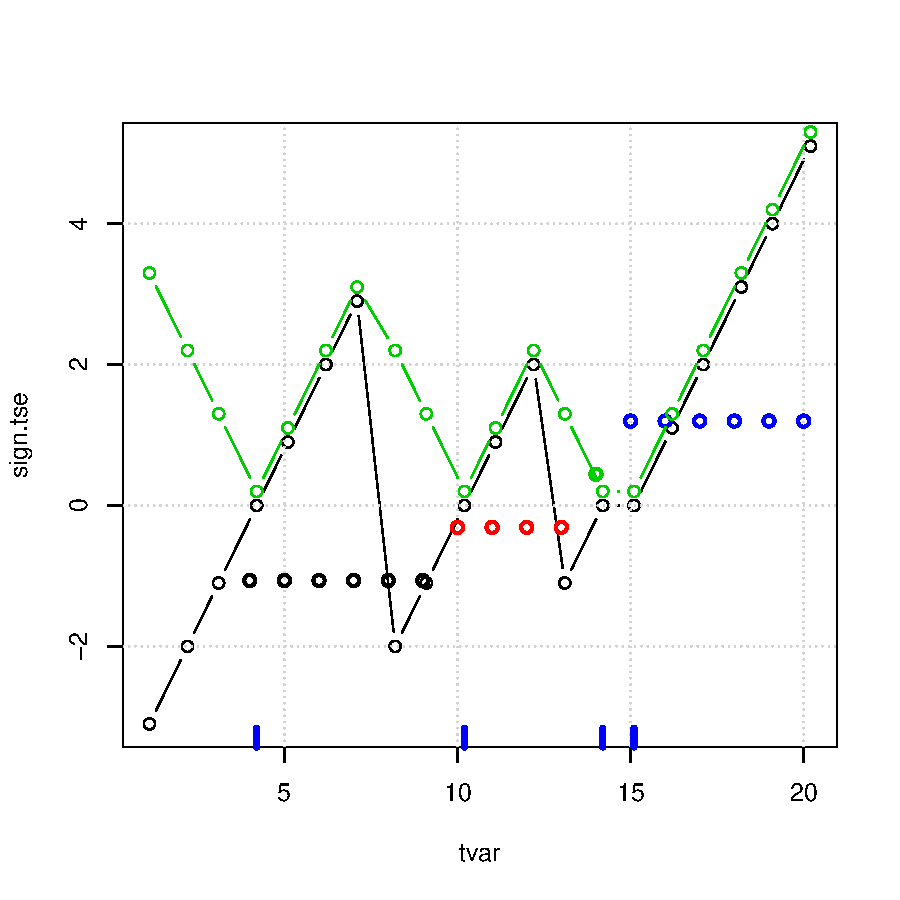
\includegraphics{figures/doBy-039}

\begin{Schunk}
\begin{Sinput}
 plot(tae~tvar, data=tse, ylim=c(-6,6),type="b")
 grid()
 lines(tbe~tvar, data=tse, type="b", col='red')
 rug(tse$tvar[tse$yvar==1], col='blue',lwd=4)
 lines(run~tvar, data=tse, col='cyan',lwd=2)
\end{Sinput}
\end{Schunk}
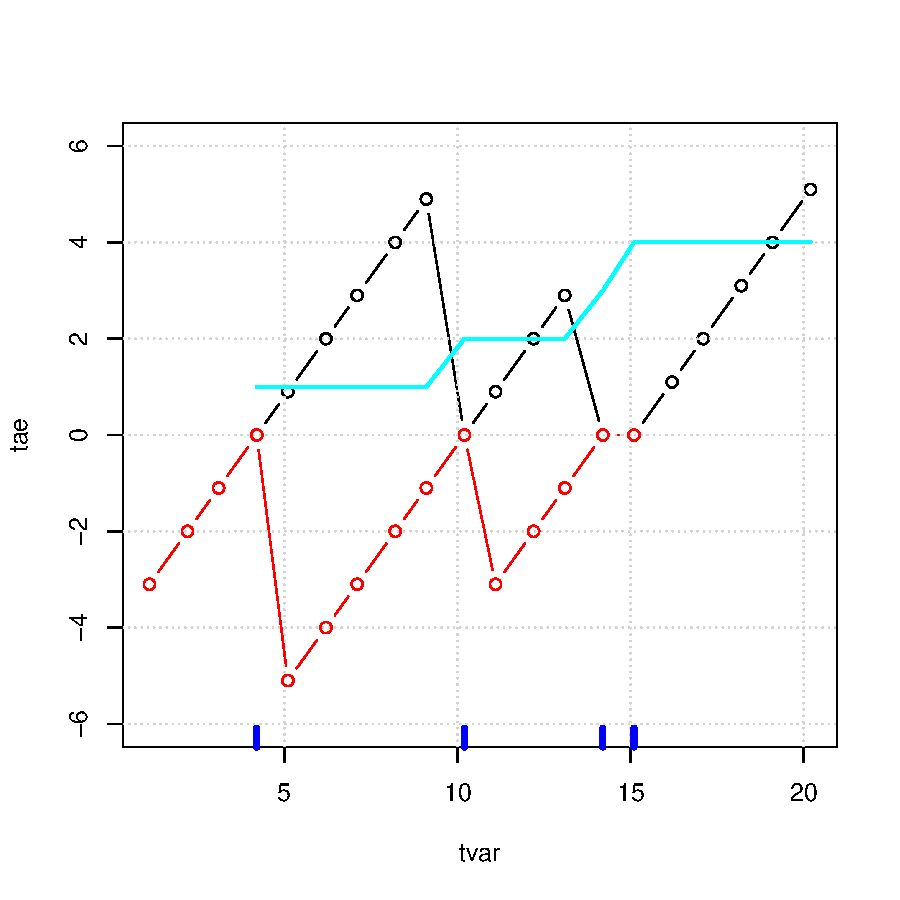
\includegraphics{figures/doBy-040}

\begin{Schunk}
\begin{Sinput}
 plot(ewin~tvar, data=tse,ylim=c(1,4))
 rug(tse$tvar[tse$yvar==1], col='blue',lwd=4)
 grid()
 lines(run~tvar, data=tse,col='red')
\end{Sinput}
\end{Schunk}
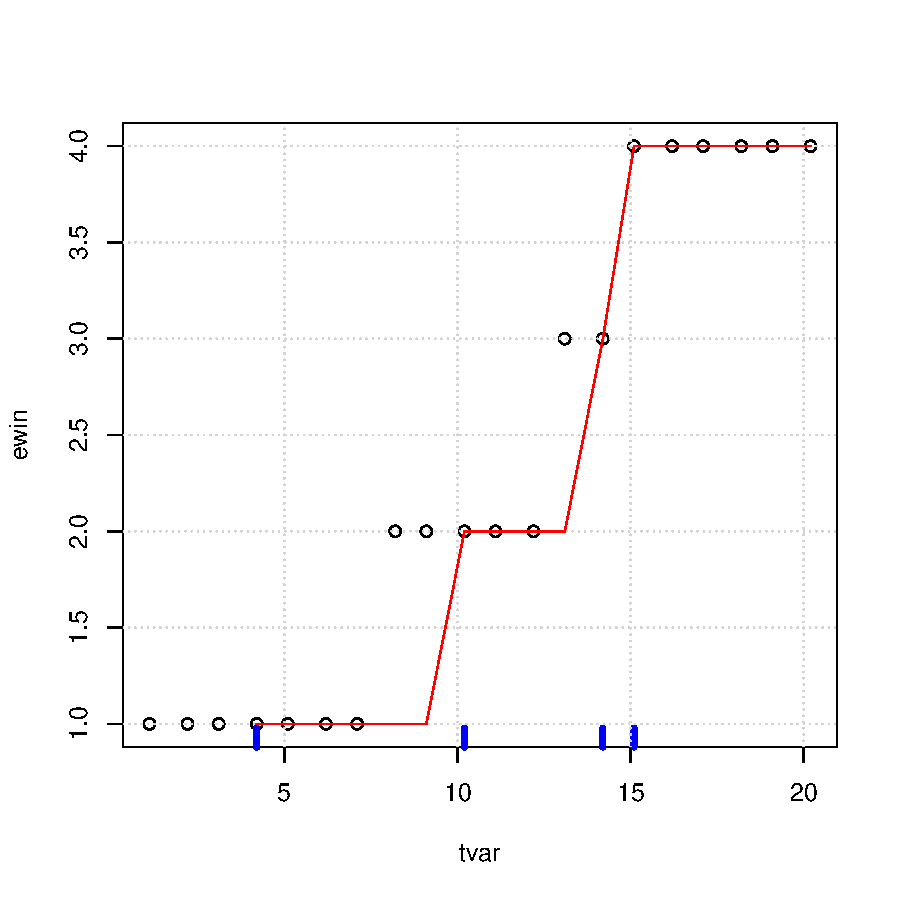
\includegraphics{figures/doBy-041}


We may now find times for which time since an event is at most 1 as
\begin{Schunk}
\begin{Sinput}
 tse$tvar[tse$abs<=1]
\end{Sinput}
\begin{Soutput}
[1]  4.2  5.1 10.2 11.1 14.2 15.1
\end{Soutput}
\end{Schunk}

\subsection{Example: Using \code{subSeq()} and \code{timeSinceEvent()}}

Consider the \verb|lynx| data:

\begin{Schunk}
\begin{Sinput}
 yvar <- as.numeric(lynx)
 tvar <- 1821:1934
 plot(tvar,yvar,type='l')
\end{Sinput}
\end{Schunk}
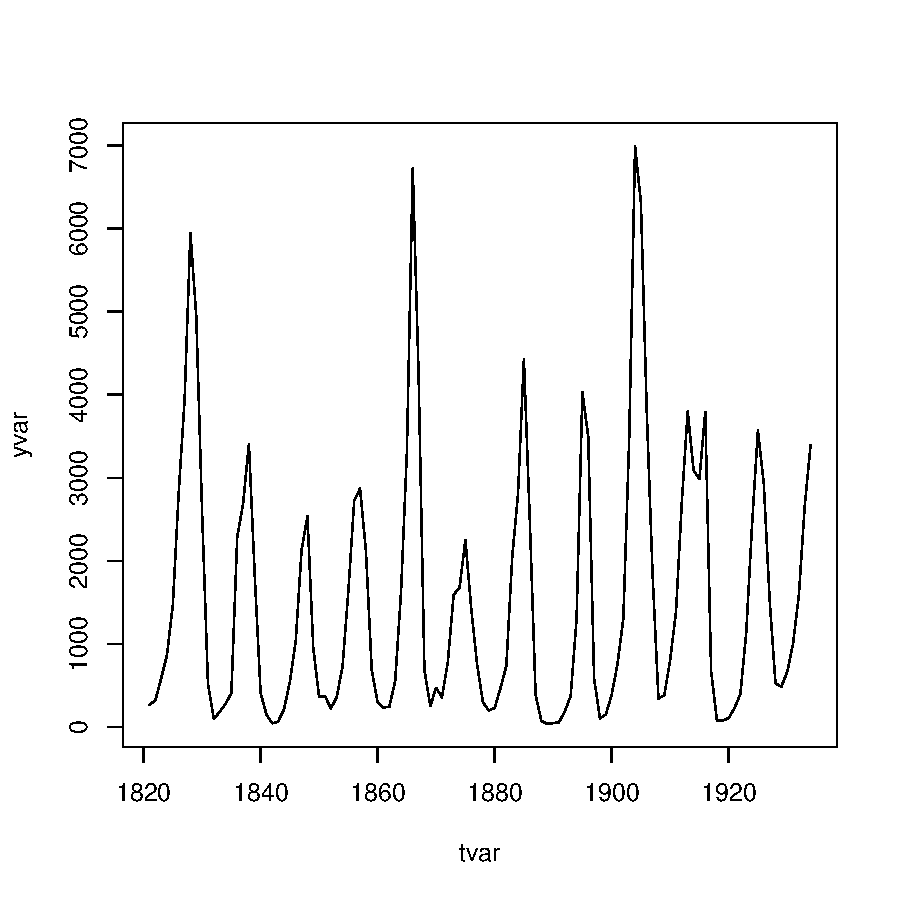
\includegraphics{figures/doBy-043}

Suppose we want to estimate the cycle lengths. One way of doing this
is as follows:

\begin{Schunk}
\begin{Sinput}
 yyy <- yvar>mean(yvar)
 head(yyy)
\end{Sinput}
\begin{Soutput}
[1] FALSE FALSE FALSE FALSE FALSE  TRUE
\end{Soutput}
\begin{Sinput}
 sss <- subSeq(yyy,TRUE)
 sss
\end{Sinput}
\begin{Soutput}
   first last slength midpoint value
1      6   10       5        8  TRUE
2     16   19       4       18  TRUE
3     27   28       2       28  TRUE
4     35   38       4       37  TRUE
5     44   47       4       46  TRUE
6     53   55       3       54  TRUE
7     63   66       4       65  TRUE
8     75   76       2       76  TRUE
9     83   87       5       85  TRUE
10    92   96       5       94  TRUE
11   104  106       3      105  TRUE
12   112  114       3      113  TRUE
\end{Soutput}
\end{Schunk}

\begin{Schunk}
\begin{Sinput}
 plot(tvar,yvar,type='l')
 rug(tvar[sss$midpoint],col='blue',lwd=4)
\end{Sinput}
\end{Schunk}
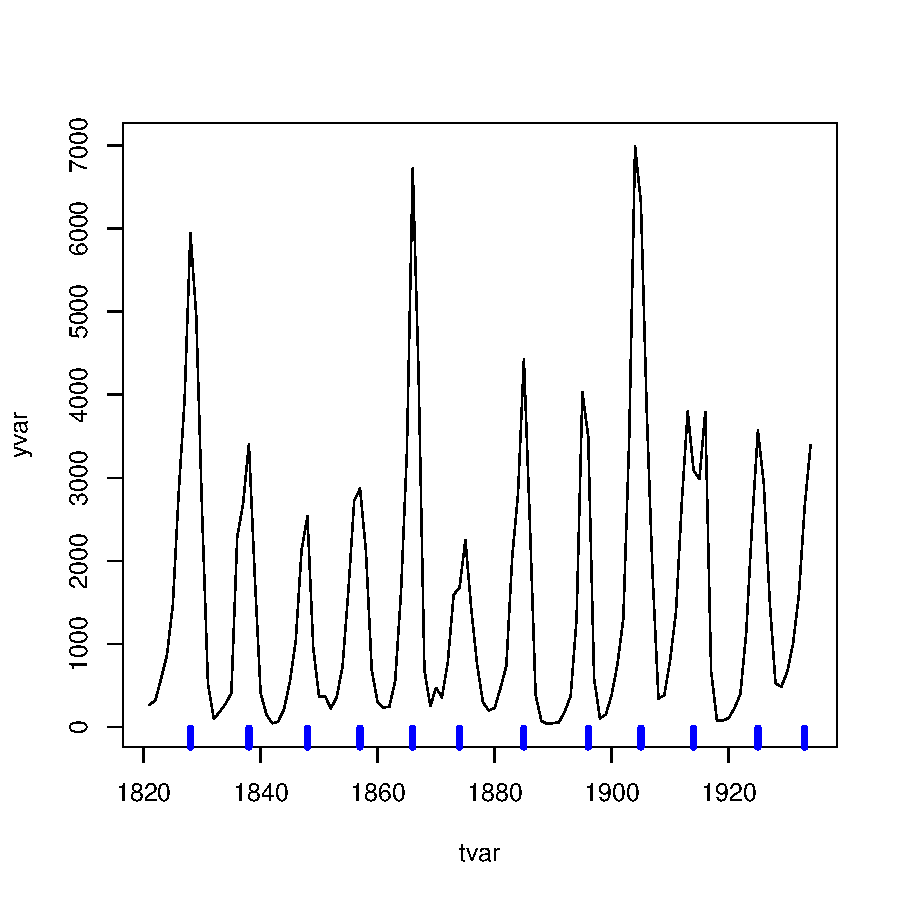
\includegraphics{figures/doBy-045}

Create the 'event vector'
\begin{Schunk}
\begin{Sinput}
 yvar2 <- rep(0,length(yvar))
 yvar2[sss$midpoint] <- 1
 str(yvar2)
\end{Sinput}
\begin{Soutput}
 num [1:114] 0 0 0 0 0 0 0 1 0 0 ...
\end{Soutput}
\end{Schunk}

\begin{Schunk}
\begin{Sinput}
 tse <- timeSinceEvent(yvar2, tvar)
 head(tse,20)
\end{Sinput}
\begin{Soutput}
   yvar tvar abs.tse sign.tse ewin run tae tbe
1     0 1821       7       -7    1  NA  NA  -7
2     0 1822       6       -6    1  NA  NA  -6
3     0 1823       5       -5    1  NA  NA  -5
4     0 1824       4       -4    1  NA  NA  -4
5     0 1825       3       -3    1  NA  NA  -3
6     0 1826       2       -2    1  NA  NA  -2
7     0 1827       1       -1    1  NA  NA  -1
8     1 1828       0        0    1   1   0   0
9     0 1829       1        1    1   1   1  -9
10    0 1830       2        2    1   1   2  -8
11    0 1831       3        3    1   1   3  -7
12    0 1832       4        4    1   1   4  -6
13    0 1833       5        5    1   1   5  -5
14    0 1834       4       -4    2   1   6  -4
15    0 1835       3       -3    2   1   7  -3
16    0 1836       2       -2    2   1   8  -2
17    0 1837       1       -1    2   1   9  -1
18    1 1838       0        0    2   2   0   0
19    0 1839       1        1    2   2   1  -9
20    0 1840       2        2    2   2   2  -8
\end{Soutput}
\end{Schunk}

We get two different (not that different) estimates of period
lengths:
\begin{Schunk}
\begin{Sinput}
 len1 <- tapply(tse$ewin, tse$ewin, length)
\end{Sinput}
\begin{Soutput}
 1  2  3  4  5  6  7  8  9 10 11 12 
13 10  9  9  9  9 11 10  9 10 10  5 
\end{Soutput}
\begin{Sinput}
 len2 <- tapply(tse$run, tse$run, length)
\end{Sinput}
\begin{Soutput}
 1  2  3  4  5  6  7  8  9 10 11 12 
10 10  9  9  8 11 11  9  9 11  8  2 
\end{Soutput}
\begin{Sinput}
 c(median(len1),median(len2),mean(len1),mean(len2))
\end{Sinput}
\begin{Soutput}
[1] 9.500 9.000 9.500 8.917
\end{Soutput}
\end{Schunk}

We can overlay the cycles as:
\begin{Schunk}
\begin{Sinput}
 tse$yvar <- yvar
 tse2 <- na.omit(tse)
 plot(yvar~tae, data=tse2)
\end{Sinput}
\end{Schunk}
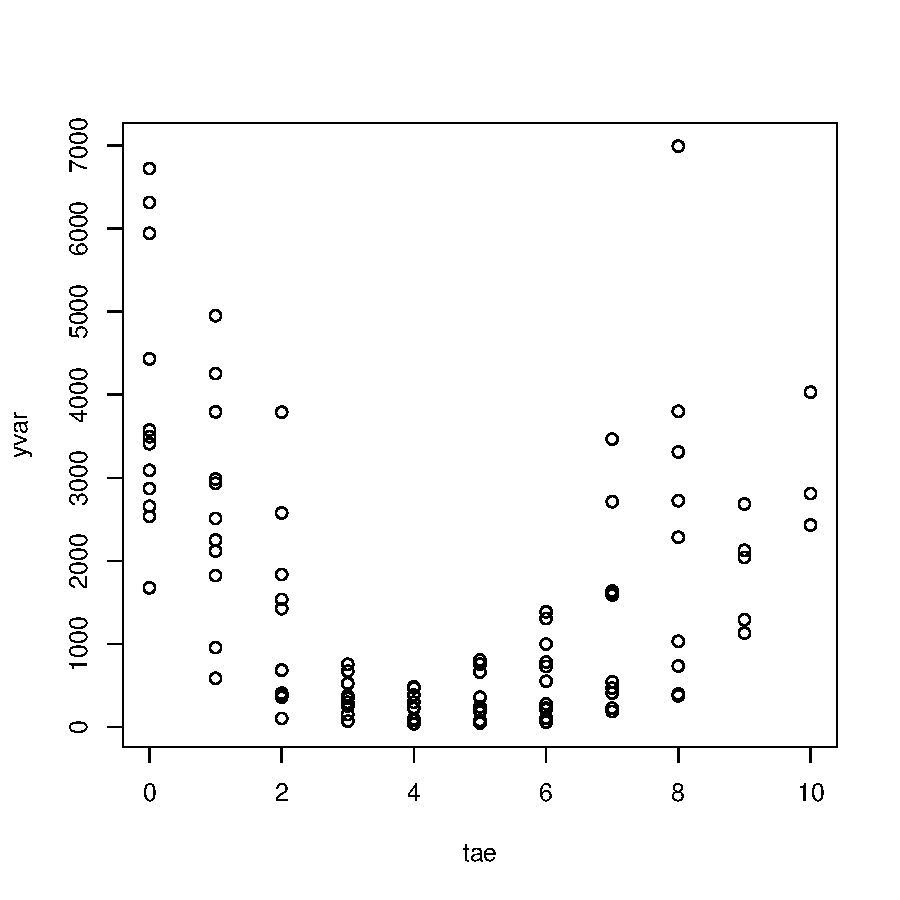
\includegraphics{figures/doBy-049}

\begin{Schunk}
\begin{Sinput}
 plot(tvar,yvar,type='l',lty=2)
 mm <- lm(yvar~tae+I(tae^2)+I(tae^3), data=tse2)
 lines(fitted(mm)~tvar, data=tse2, col='red')
\end{Sinput}
\end{Schunk}
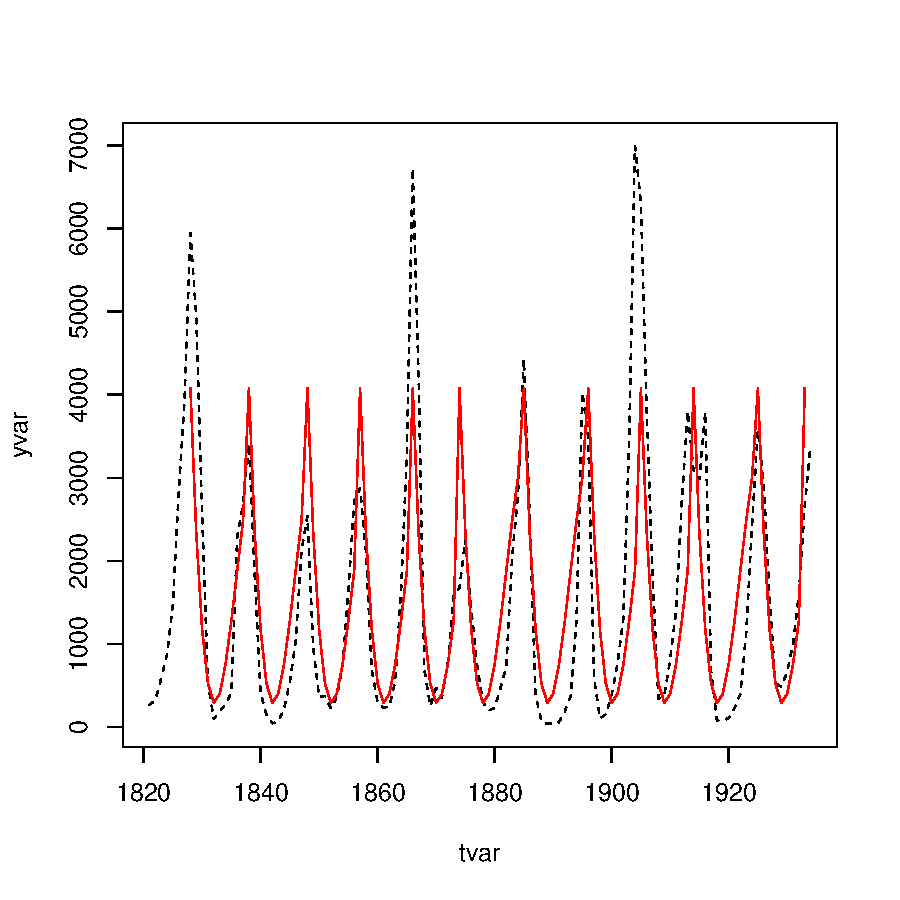
\includegraphics{figures/doBy-050}


% \section{Acknowledgements}
% \label{discussion}

% Credit is due to
% Dennis Chabot, Gabor Grothendieck, Paul Murrell, Jim Robison-Cox  and Erik J{\o}rgensen for
% reporting various bugs and making various suggestions to the
% functionality in the \doby{} package.



\end{document}



\appendix

\section{The data}
\label{sec:appdata}

The reduced \code{C02} are:
\begin{Schunk}
\begin{Sinput}
> CO2
\end{Sinput}
\begin{Soutput}
   Plant Type conc uptake Treat
1    Qn1  Que   95   16.0 nchil
2    Qn1  Que  175   30.4 nchil
3    Qn1  Que  250   34.8 nchil
4    Qn1  Que  350   37.2 nchil
5    Qn1  Que  500   35.3 nchil
6    Qn1  Que  675   39.2 nchil
7    Qn1  Que 1000   39.7 nchil
22   Qc1  Que   95   14.2  chil
23   Qc1  Que  175   24.1  chil
24   Qc1  Que  250   30.3  chil
25   Qc1  Que  350   34.6  chil
26   Qc1  Que  500   32.5  chil
27   Qc1  Que  675   35.4  chil
28   Qc1  Que 1000   38.7  chil
43   Mn1  Mis   95   10.6 nchil
44   Mn1  Mis  175   19.2 nchil
45   Mn1  Mis  250   26.2 nchil
46   Mn1  Mis  350   30.0 nchil
47   Mn1  Mis  500   30.9 nchil
48   Mn1  Mis  675   32.4 nchil
49   Mn1  Mis 1000   35.5 nchil
64   Mc1  Mis   95   10.5  chil
65   Mc1  Mis  175   14.9  chil
66   Mc1  Mis  250   18.1  chil
67   Mc1  Mis  350   18.9  chil
68   Mc1  Mis  500   19.5  chil
69   Mc1  Mis  675   22.2  chil
70   Mc1  Mis 1000   21.9  chil
\end{Soutput}
\end{Schunk}

The reduced \code{airquality} data are:
\begin{Schunk}
\begin{Sinput}
> head(airquality, n=20)
\end{Sinput}
\begin{Soutput}
   Ozone Solar.R Wind Temp Month Day
1     41     190  7.4   67     5   1
2     36     118  8.0   72     5   2
3     12     149 12.6   74     5   3
4     18     313 11.5   62     5   4
5     NA      NA 14.3   56     5   5
6     28      NA 14.9   66     5   6
7     23     299  8.6   65     5   7
8     19      99 13.8   59     5   8
9      8      19 20.1   61     5   9
10    NA     194  8.6   69     5  10
11     7      NA  6.9   74     5  11
12    16     256  9.7   69     5  12
13    11     290  9.2   66     5  13
14    14     274 10.9   68     5  14
15    18      65 13.2   58     5  15
16    14     334 11.5   64     5  16
17    34     307 12.0   66     5  17
18     6      78 18.4   57     5  18
19    30     322 11.5   68     5  19
20    11      44  9.7   62     5  20
\end{Soutput}
\end{Schunk}
